\documentclass{article}
\usepackage[utf8]{inputenc}

\usepackage{tikz}
\usetikzlibrary{positioning, fit}

\begin{document}

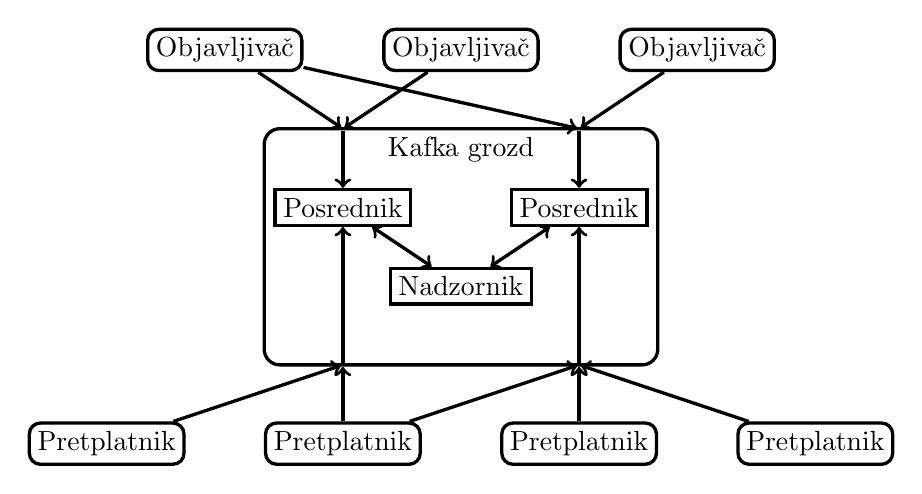
\begin{tikzpicture}[ % has a lot of options; consult the pgf manual
bend angle=45,
long_square/.style={rectangle, draw=black, fill=white, very thick, inner sep=3pt, minimum width=14mm},
rounded_square/.style={rectangle, rounded corners, draw=black, fill=white, very thick, inner sep=3pt, minimum width=14mm},
empty_circle/.style={rectangle, rounded corners=2mm, draw=black, fill=white, very thick, minimum size=4mm},
point/.style={circle, inner sep=0mm},
fit_square/.style={rectangle, rounded corners=2mm, draw=black, very thick, minimum height=30mm},
both_arrow/.style={<->, very thick},
out_arrow/.style={->, very thick},
in_arrow/.style={<-, very thick},
above_edge_text/.style={above, midway, sloped}
]

\node[rounded_square](prod_1) at (1.5,0) {Objavljivač};
\node[rounded_square](prod_2) at (4.5,0) {Objavljivač};
\node[rounded_square](prod_3) at (7.5,0) {Objavljivač};

\node[point](entry_1) at (3,-1) {};
\node[point](entry_2) at (6,-1) {};

\node[long_square](broker_1) at (3,-2) {Posrednik};
\node[long_square](broker_2) at (6,-2) {Posrednik};

\node[long_square](zookeeper) at (4.5,-3) {Nadzornik};

\node[point](exit_1) at (3,-4) {};
\node[point](exit_2) at (6,-4) {};

\node[rounded_square](cons_1) at (0,-5) {Pretplatnik};
\node[rounded_square](cons_2) at (3,-5) {Pretplatnik};
\node[rounded_square](cons_3) at (6,-5) {Pretplatnik};
\node[rounded_square](cons_4) at (9,-5) {Pretplatnik};

\node[fit_square, fit=(broker_1) (broker_2) (zookeeper)] (cluster) {};
\node[anchor=north] at (cluster.north) {Kafka grozd};



\draw[out_arrow](prod_1) to [] node[auto]{} (entry_1);
\draw[out_arrow](prod_1) to [] node[auto]{} (entry_2);
\draw[out_arrow](prod_2) to [] node[auto]{} (entry_1);
\draw[out_arrow](prod_3) to [] node[auto]{} (entry_2);

\draw[out_arrow](entry_1) to [] node[auto]{} (broker_1);
\draw[out_arrow](entry_2) to [] node[auto]{} (broker_2);

\draw[both_arrow](zookeeper) to [] node[auto]{} (broker_1);
\draw[both_arrow](zookeeper) to [] node[auto]{} (broker_2);

\draw[out_arrow](exit_1) to [] node[auto]{} (broker_1);
\draw[out_arrow](exit_2) to [] node[auto]{} (broker_2);

\draw[out_arrow](cons_1) to [] node[auto]{} (exit_1);
\draw[out_arrow](cons_2) to [] node[auto]{} (exit_1);
\draw[out_arrow](cons_2) to [] node[auto]{} (exit_2);
\draw[out_arrow](cons_3) to [] node[auto]{} (exit_2);
\draw[out_arrow](cons_4) to [] node[auto]{} (exit_2);

\end{tikzpicture}

\end{document}